% !TEX program = XeLaTeX
%----------------------------------------------------------------------------------------
% PACKAGES
%----------------------------------------------------------------------------------------
\documentclass[hyperref={pdfpagelabels=false}]{beamer}
\usepackage[orientation=portrait,size=a0,scale=1.15]{beamerposter}
\usepackage[font={small}]{caption}
\usepackage[english]{babel}
\usepackage{amsmath, booktabs, fontspec, graphicx, xcolor, tikz, tabularx}
\usetikzlibrary{arrows.meta, positioning, shapes.geometric}

%----------------------------------------------------------------------------------------
% DOCUMENT CONFIGURATIONS
%----------------------------------------------------------------------------------------
\usetheme{NTNU}

\setlength{\paperwidth}{33.1in}
\setlength{\paperheight}{46.8in}

\captionsetup{skip=0pt, belowskip=0pt, aboveskip=0pt, font=small}
\setbeamertemplate{caption}[numbered]

\setmainfont[
  Path=resources/fonts/,
  Extension=.ttf,
  BoldFont=*bd,
  ItalicFont=*i,
  BoldItalicFont=*bi
]{arial}
\setsansfont[
  Path=resources/fonts/,
  Extension=.ttf,
  BoldFont=*bd,
  ItalicFont=*i,
  BoldItalicFont=*bi
]{arial}

\newlength\origleftmargini
\setlength\origleftmargini\leftmargini
\setbeamertemplate{itemize/enumerate body begin}{\setlength{\leftmargini}{1.2em}}

\definecolor{ntnublue}{HTML}{00509E}
\definecolor{resultgreen}{HTML}{00843D}
\definecolor{warnred}{HTML}{C64632}
\definecolor{softgray}{HTML}{EEF2F5}
\definecolor{darkgray}{HTML}{232834}

\newcommand{\keymetric}[3]{%
  \begin{tikzpicture}
    \node[
      rounded corners=4pt,
      draw=#1,
      line width=1.2pt,
      fill=#1!8,
      inner sep=10pt,
      text width=0.28\columnwidth,
      align=center
      
    ] {\Large\textbf{#2}\\[0.3em]\normalsize #3};
  \end{tikzpicture}%
}

%----------------------------------------------------------------------------------------
% TITLE SECTION
%----------------------------------------------------------------------------------------
\title{\huge{Real-Time Impact Point Prediction of Suborbital Rockets\\Using Kalman Filtering}}

\author{Emil Killingberg Jensen, Kristoffer Gryte}

\institute{\normalsize\texttt{emilkj@stud.ntnu.no} \quad $|$ \quad \texttt{kristoffer.gryte@ntnu.no} \\[0.4em]
Department of Engineering Cybernetics, NTNU}

%----------------------------------------------------------------------------------------

\begin{document}

\addtobeamertemplate{block end}{}{\vspace*{1ex}}

\begin{frame}[fragile]
\begin{columns}[t]

%----------------------------------------------------------------------------------------
% FIRST COLUMN
%----------------------------------------------------------------------------------------
\begin{column}{.052\textwidth}\end{column}

\begin{column}{.45\textwidth}

\begin{block}{Motivation}
  Rocket launch rates are rising. Recovering payloads and first stages using autonomous
  recovery vehicles (ARVs) reduces cost, human exposure, and environmental footprint.
  The challenge is knowing where the rocket will land \textit{before it gets there}.

  \vspace{0.5em}
  \textbf{Impact point prediction (IPP)} is the real-time estimate of the rocket's
  landing location and uncertainty, updated continuously from onboard sensor data.
  An ARV steers to this estimate.

  \vspace{0.6em}
  \begin{center}
  \begin{tikzpicture}[
    font=\small,
    physbox/.style={rectangle, rounded corners=5pt, draw=darkgray, line width=1.2pt,
                    fill=white, align=center, text width=5.0cm, minimum height=3.0cm},
    algbox/.style={rectangle, rounded corners=5pt, draw=ntnublue, line width=1.6pt,
                   fill=ntnublue!8, align=center, text width=3.0cm, minimum height=2.0cm},
    ippbox/.style={algbox, draw=resultgreen, fill=resultgreen!8},
    arrow/.style={-{Latex[length=4mm, width=3mm]}, line width=1.3pt, draw=darkgray},
    datatag/.style={font=\scriptsize, align=center, rounded corners=3pt,
                    fill=darkgray!8, draw=darkgray!35, line width=0.5pt,
                    inner xsep=5pt, inner ysep=3pt},
    navtag/.style={datatag, fill=ntnublue!10, draw=ntnublue!40},
    ipptag/.style={datatag, fill=resultgreen!10, draw=resultgreen!40}
  ]
    % Softgray module background — drawn first so nodes render on top
    \draw[rounded corners=8pt, draw=darkgray!50, line width=1.0pt, fill=softgray!60]
      (-5.5cm, 3.6cm) rectangle (5.5cm, -3.6cm);
    \node[font=\scriptsize\itshape, text=darkgray!70] at (0cm, 4.1cm)
      {\textit{Onboard algorithm}};

    % Algorithm nodes — spread apart to leave room for the nav state label between them
    \node[algbox] (eskf) at (0cm,  2.2cm) {\textbf{ESKF}};
    \node[ippbox] (ipp)  at (0cm, -2.2cm) {\textbf{IPP EKF}};

    % Physical entities at mid-height (y=0)
    \node[physbox] (rocket)  at (-12.5cm, 0) {\textbf{Rocket}};
    \node[physbox] (vehicle) at ( 12.5cm, 0) {\textbf{ARV}};

    % External arrows — straight horizontal at y=0
    \draw[arrow] (rocket.east) -- (-5.5cm, 0)
      node[midway, above=3pt, datatag] {sensor data};
    \draw[arrow] (5.5cm, 0) -- (vehicle.west)
      node[midway, above=3pt, ipptag] {impact point\\+ covariance};

    % Internal arrow — nav state label centred in the gap between the two blocks
    \draw[arrow] (eskf.south) -- (ipp.north);
    \node[navtag, anchor=west] at (0.15cm, 0cm) {Navigation state\\and covariance};
  \end{tikzpicture}
  \end{center}

\end{block}

\begin{block}{System \& Method}

  \textbf{Navigation — Error-State Kalman Filter (ESKF)}

  \vspace{0.3em}
  The ESKF maintains a continuous estimate of position, velocity, attitude, and sensor
  biases. IMU measurements propagate the state at high rate. GNSS, barometer, and
  magnetometer measurements then correct it via the error-state injection scheme~[3].
  The filter outputs a full state vector \textit{and covariance} that are passed directly
  as the initial condition for the IPP filter.

  \vspace{0.8em}
  \textbf{Impact Point Prediction — Cartesian EKF}

  \vspace{0.3em}
  The IPP filter propagates a Cartesian state
  $\mathbf{x} = [\mathbf{p}^\top, \mathbf{v}^\top]^\top$ in NED coordinates forward
  until altitude reaches sea level:

  \vspace{0.2em}
  \begin{center}
  \begin{minipage}{0.97\columnwidth}
  \begin{equation*}
    \dot{\mathbf{p}} = \mathbf{v}, \qquad
    \dot{\mathbf{v}} = \mathbf{g}
      - K_D\,\mathbf{v}_a
      + \mathbf{R}(\hat{\mathbf{q}})\,\mathbf{T}_b, \qquad
    K_D = \frac{\rho\, C_D\, A\,\|\mathbf{v}_a\|}{2m}
  \end{equation*}
  \end{minipage}
  \end{center}

  \vspace{0.2em}
  $\mathbf{v}_a$ airspeed vector, $\rho$ air density, $C_D$ drag coefficient, $A$ reference area, $m$ mass.
  $\mathbf{R}(\hat{\mathbf{q}})$ rotates the body-frame thrust $\mathbf{T}_b$ to NED using the ESKF attitude quaternion $\hat{\mathbf{q}}$.

  \vspace{0.3em}
  The equations are propagated forward until the predicted altitude reaches sea level,
  yielding a predicted impact point and propagated uncertainty ellipse updated in real time.

  \vspace{0.8em}
  \begin{tabularx}{0.97\columnwidth}{>{\bfseries}l X}
    \toprule
    Component & Key design choice \\
    \midrule
    ESKF & Fuses GNSS, barometer, and magnetometer \\
    IPP  & Forward propagation of position and velocity using EKF equations \\
    Interface & IPP re-initialised from ESKF state and covariance at each GNSS update \\
    \bottomrule
  \end{tabularx}

\end{block}

\end{column}

%----------------------------------------------------------------------------------------
% SECOND COLUMN
%----------------------------------------------------------------------------------------
\begin{column}{.01\textwidth}\end{column}

\begin{column}{.45\textwidth}

\begin{block}{Results: Real-Flight Validation}
  % PLACEHOLDER — replace with geographic map figure once generated
  % (predicted impact track converging to actual landing point)
  The figure compares horizontal IPP error from a real Andøya student-rocket launch against
  a representative simulated trajectory. The two are distinct flights — the comparison shows
  that the error characteristics seen in simulation transfer to the real-flight setting.

  \vspace{0.4em}
  \begin{center}
    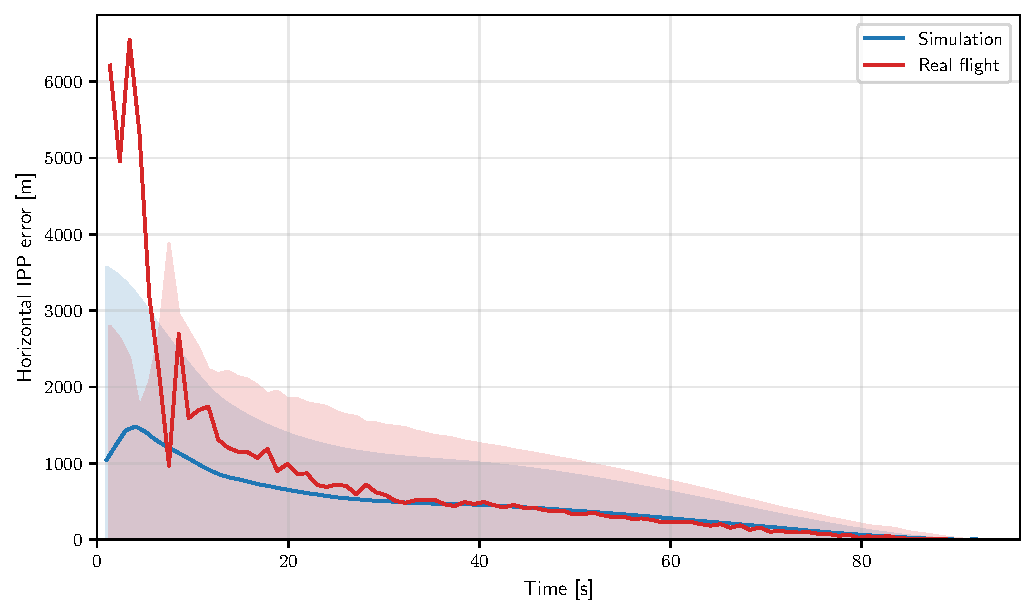
\includegraphics[width=0.95\columnwidth]{figures/sim_vs_real_ipp_error.pdf}
  \end{center}

  \vspace{0.3em}
  During the powered phase ($t \lesssim 10$~s) the prediction carries high uncertainty due
  to gyroscope saturation from peak spin rates. After motor burnout, the filter produces
  stable predictions with low and well-bounded horizontal error throughout the full 80~s
  descent to splashdown.
\end{block}


\begin{block}{Challenges \& Outlook}
  \begin{itemize}
    \item \textbf{Powered-phase limitation:} peak spin rate of ${\approx}$113~rad/s
          exceeds the gyroscope range, saturating the IMU during boost.
          A higher-range gyroscope and repositioning the IMU closer to the spin axis would address this.
    \item \textbf{Wind and drag uncertainty:} real-time wind estimation and
          in-flight drag identification remain open problems for operational use.
    \item \textbf{Known mass and thrust:} the IPP model treats vehicle mass and thrust
          as deterministic inputs. Propellant burn-off and thrust variations introduce
          unmodelled uncertainty that limits pre-burnout accuracy; in-flight parameter
          estimation would address this.
    \item \textbf{Scaling to orbital recovery:} the ESKF--Cartesian architecture
          requires only higher-grade inertial sensors and a longer propagation
          horizon to support autonomous ship pre-positioning before first-stage
          splashdown.
  \end{itemize}
\end{block}

\begin{block}{References}
  \small
  \begin{tabular}{@{}r@{\hspace{0.5em}}p{0.87\columnwidth}@{}}
    {[1]} & K.~Gryte et al.
            \textit{Recovery of Rocket Payloads and First Stages Using Unmanned Vehicles.}
            IEEE Aerospace Conference, 2025. \\[0.4em]
    {[2]} & A.~Meta.
            \textit{Impact Point Prediction of High-Power Rockets and Sounding Rockets.}
            M.Sc.\ Thesis, NTNU, 2025. \\[0.4em]
    {[3]} & E.~K.~Jensen.
            \textit{Impact Point Prediction of High-Power Rockets and Sounding Rockets.}
            M.Sc.\ Thesis, NTNU, 2026. \\
  \end{tabular}
\end{block}

\end{column}

\begin{column}{.039\textwidth}\end{column}

\end{columns}
\end{frame}

\end{document}
